% \begin{minipage}{0.5\textwidth}
\begin{figure}[t]
    \centering
    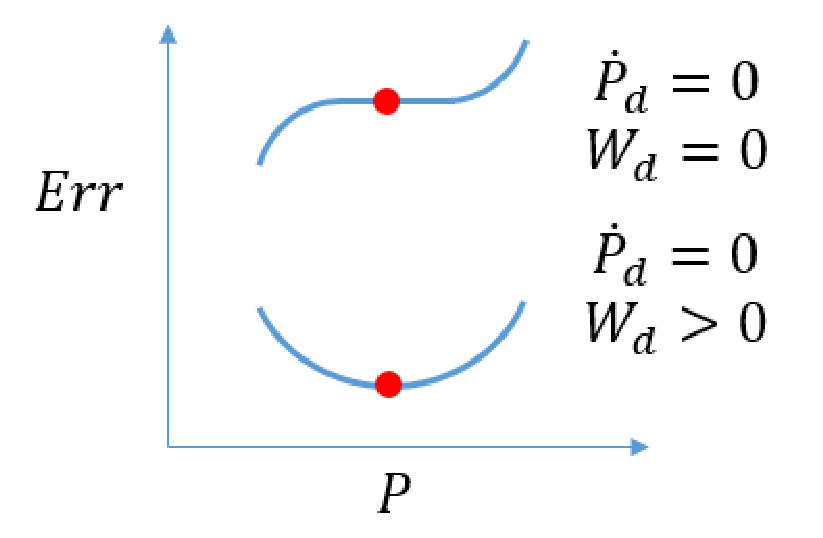
\includegraphics[width=1.8in]{error_graphs_modified}
    \caption{Top Line: moving the point does not change the error, thus the desired movement is zero, however, it is not important to achieve zero movement, thus $W_d = 0$.  Bottom Line: error is at a local minimum; thus moving the point increases error.}
    % \vspace{-0.2in}
    \label{fig:error_examples}
\end{figure}
% \end{minipage}